%&pdfLaTeX
% !TEX encoding = UTF-8 Unicode
\documentclass{article}
\usepackage{ifxetex}
\ifxetex
\usepackage{fontspec}
\setmainfont[Mapping=tex-text]{STIXGeneral}
\else
\usepackage[T1]{fontenc}
\usepackage[utf8]{inputenc}
\fi
\usepackage{textcomp}

\usepackage{graphicx}
\usepackage{array}
\usepackage{amssymb}
\usepackage[T2A]{fontenc}
\usepackage[russian]{babel}
\usepackage{fancyhdr}
\renewcommand{\headrulewidth}{0pt}
\renewcommand{\footrulewidth}{0pt}
\usepackage{color}

\definecolor{color17}{rgb}{0.31,0.51,0.74}

\begin{document}

\vspace{10pt}
\subsubsection*{{\color{color17} \textbf{1.2.2 Радиальная часть}}}

\vspace{10pt}
\baselineskip=18pt
{\large{}Т.к. уравнение на радиальную часть как 
в кулоновском, как и в кулон-дипольном случае 
можно свести к уравнению на фукцию Уитеккера, 
рассмотрим некоторые свойства этих функций, 
которые в дальнейшем будут нам полезны.\label{HToc453749984}}

\vspace{10pt}
\baselineskip=13pt
{\color{color17} \textit{\textbf{1.2.2.1 Свойства M- и W- функций 
Уитеккера[9]}}}

\vspace{10pt}
\baselineskip=18pt
{\large{}а) Уравнение на функции}

\vspace{10pt}
%%\begin{figure}[htbp]
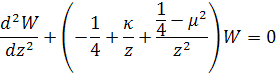
\includegraphics[width=208pt, height=58pt, keepaspectratio=true]{3-fig001.png}
%%\caption{This should be the caption for \texttt{3-fig001.png}.}
%%\end{figure}

\vspace{28pt}
{\large{}б) }
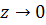
\includegraphics[width=35pt, height=19pt, keepaspectratio=true]{3-fig002.png}

\vspace{10pt}
%%\begin{figure}[htbp]
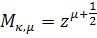
\includegraphics[width=73pt, height=29pt, keepaspectratio=true]{3-fig003.png}
%%\caption{This should be the caption for \texttt{3-fig003.png}.}
%%\end{figure}

\vspace{28pt}
{\large{}В случае, если }
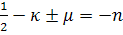
\includegraphics[width=92pt, height=26pt, keepaspectratio=true]{3-fig004.png}

\vspace{10pt}
%%\begin{figure}[htbp]
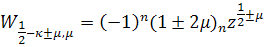
\includegraphics[width=199pt, height=35pt, keepaspectratio=true]{3-fig005.png}
%%\caption{This should be the caption for \texttt{3-fig005.png}.}
%%\end{figure}

\vspace{28pt}
{\large{}Иначе}

\vspace{10pt}
%%\begin{figure}[htbp]
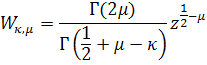
\includegraphics[width=155pt, height=49pt, keepaspectratio=true]{3-fig006.png}
%%\caption{This should be the caption for \texttt{3-fig006.png}.}
%%\end{figure}

\vspace{28pt}
{\large{}в) }
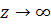
\includegraphics[width=38pt, height=19pt, keepaspectratio=true]{3-fig007.png}

\vspace{10pt}
%%\begin{figure}[htbp]
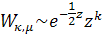
\includegraphics[width=77pt, height=29pt, keepaspectratio=true]{3-fig008.png}
%%\caption{This should be the caption for \texttt{3-fig008.png}.}
%%\end{figure}

\vspace{28pt}
{\large{}В случае, если }
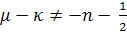
\includegraphics[width=95pt, height=26pt, keepaspectratio=true]{3-fig009.png}

\vspace{10pt}
%%\begin{figure}[htbp]
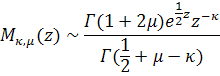
\includegraphics[width=165pt, height=57pt, keepaspectratio=true]{3-fig010.png}
%%\caption{This should be the caption for \texttt{3-fig010.png}.}
%%\end{figure}

\label{HToc453749985}

\vspace{28pt}
\baselineskip=13pt
{\color{color17} \textit{\textbf{1.2.2.2 Теоретический вывод 
радиальной функции}}}

\vspace{10pt}
\baselineskip=18pt
{\large{}Рассмотрим радиальное уравнение. }

\vspace{10pt}
%%\begin{figure}[htbp]
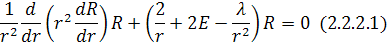
\includegraphics[width=290pt, height=35pt, keepaspectratio=true]{3-fig011.png}
%%\caption{This should be the caption for \texttt{3-fig011.png}.}
%%\end{figure}

\vspace{28pt}
{\large{}Легко можно видеть, что по виду оно абсолютно 
аналогично соответствующему кулоновскому 
уравнению, с заменой }
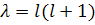
\includegraphics[width=71pt, height=19pt, keepaspectratio=true]{3-fig012.png}
{\large{}. }

\includegraphics[width=8pt, height=19pt, keepaspectratio=true]{3-fig013.png}
{\large{} - собственное значение уравнения на угловую 
часть. Соответственно, решения будут такие 
же по виду. }

\vspace{10pt}
%%\begin{figure}[htbp]
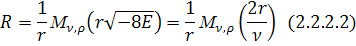
\includegraphics[width=267pt, height=35pt, keepaspectratio=true]{3-fig014.png}
%%\caption{This should be the caption for \texttt{3-fig014.png}.}
%%\end{figure}

\vspace{28pt}
%%\begin{figure}[htbp]
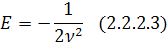
\includegraphics[width=125pt, height=34pt, keepaspectratio=true]{3-fig015.png}
%%\caption{This should be the caption for \texttt{3-fig015.png}.}
%%\end{figure}

\vspace{28pt}
%%\begin{figure}[htbp]
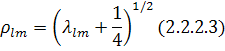
\includegraphics[width=169pt, height=38pt, keepaspectratio=true]{3-fig016.png}
%%\caption{This should be the caption for \texttt{3-fig016.png}.}
%%\end{figure}

\vspace{28pt}
{\large{}Введем понятие }
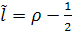
\includegraphics[width=54pt, height=26pt, keepaspectratio=true]{3-fig017.png}
{\large{} - квазиугловой момент.}

\vspace{10pt}
{\large{}Приведем таблицу значений }

\includegraphics[width=5pt, height=20pt, keepaspectratio=true]{3-fig018.png}
{\large{} в зависимости от значений дипольного 
момента}

\vspace{10pt}
\begin{tabular}{|>{\raggedright}p{37pt}|>{\raggedright}p{39pt}|>{\raggedright}p{35pt}|>{\raggedright}p{35pt}|>{\raggedright}p{41pt}|>{\raggedright}p{35pt}|>{\raggedright}p{36pt}|}
\hline
d & \multicolumn{3}{p{111pt}|}{m\textit{ (unknown char) 0}} & \multicolumn{2}{p{76pt}|}{m\textit{ 
(unknown char) 1}} & m\textit{ (unknown char) 2}\tabularnewline
\hline
 & l\textit{ (unknown char) 0} & l\textit{ (unknown char) 1} & l\textit{ (unknown char) 
2} & l\textit{ (unknown char) 1} & l\textit{ (unknown char) 2} & l\textit{ (unknown char) 
2}\tabularnewline
\hline
0,2 & -0,02715 & 1,00524 & 2,00076 & 0,997334 & 2,00038 & 1,99924\tabularnewline
\hline
0,4 & -0,11636 & 1,01989 & 2,00306 & 0,989341 & 2,0015 & 1,99695\tabularnewline
\hline
0,6 & -0,33328 & 1,04134 & 2,00694 & 0,976038 & 2,00329 & 1,99315\tabularnewline
\hline
0,8 & - & 1,06655 & 2,01244 & 0,957442 & 2,00567 & 1,98783\tabularnewline
\hline
1,0 & - & 1,09285 & 2,01961 & 0,933563 & 2,00851 & 1,98101\tabularnewline
\hline
1,2 & - & 1,11824 & 2,02852 & 0,904393 & 2,01168 & 1,97268\tabularnewline
\hline
1,4 & - & 1,1413 & 2,03918 & 0,869881 & 2,01501 & 1,96287\tabularnewline
\hline
1,6 & - & 1,16111 & 2,05158 & 0,829924 & 2,01835 & 1,95158\tabularnewline
\hline
1,8 & - & 1,17709 & 2,06566 & 0,784337 & 2,02156 & 1,93883\tabularnewline
\hline
2,0 & - & 1,1889 & 2,08132 & 0,732823 & 2,02448 & 1,92462\tabularnewline
\hline
\end{tabular}

\vspace{10pt}
\begin{center}
Таблица 1.
\end{center}

\vspace{10pt}
\baselineskip=18pt
\leftskip=0pt
{\large{}Для того, чтобы выполнялись граничные 
условия при }
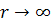
\includegraphics[width=38pt, height=19pt, keepaspectratio=true]{3-fig019.png}
{\large{}, необходимо, чтобы между }

\includegraphics[width=8pt, height=19pt, keepaspectratio=true]{3-fig020.png}
{\large{} и }

\includegraphics[width=8pt, height=19pt, keepaspectratio=true]{3-fig021.png}
{\large{} выполнялось соотношение (см. свойство 
(в) п. 1.2.2.1).}

\vspace{10pt}
%%\begin{figure}[htbp]
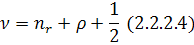
\includegraphics[width=146pt, height=34pt, keepaspectratio=true]{3-fig022.png}
%%\caption{This should be the caption for \texttt{3-fig022.png}.}
%%\end{figure}

\vspace{28pt}
{\large{}Учитывая, что }
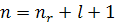
\includegraphics[width=87pt, height=19pt, keepaspectratio=true]{3-fig023.png}
{\large{}, }
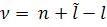
\includegraphics[width=80pt, height=20pt, keepaspectratio=true]{3-fig024.png}

\vspace{10pt}
{\large{}Для квантового дефекта тогда получим выражение}
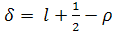
\includegraphics[width=85pt, height=26pt, keepaspectratio=true]{3-fig025.png}

\vspace{10pt}
{\large{}При использовании исключительно теоретических 
построений возникает следующая проблема: рассчитанные 
квантовые дефекты включают в себя только дипольную 
часть и не учитывают короткодействующую часть 
потенциала.}

\vspace{10pt}
%%\begin{figure}[htbp]
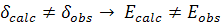
\includegraphics[width=166pt, height=19pt, keepaspectratio=true]{3-fig026.png}
%%\caption{This should be the caption for \texttt{3-fig026.png}.}
%%\end{figure}

\label{HToc453749986}

\vspace{28pt}
\baselineskip=13pt
{\color{color17} \textit{\textbf{1.2.2.3 Модельный потенциал 
Саймонса }}}

\vspace{10pt}
\baselineskip=18pt
{\large{}Эмпирически наблюдаемый квантовый дефект 
можно учесть, рассматривая модельный потенциал 
следующего вида[10]:}

\vspace{10pt}
%%\begin{figure}[htbp]
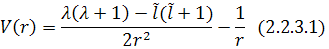
\includegraphics[width=247pt, height=37pt, keepaspectratio=true]{3-fig027.png}
%%\caption{This should be the caption for \texttt{3-fig027.png}.}
%%\end{figure}

\vspace{28pt}
%%\begin{figure}[htbp]

\includegraphics[width=8pt, height=19pt, keepaspectratio=true]{3-fig028.png}
%%\caption{This should be the caption for \texttt{3-fig028.png}.}
%%\end{figure}

 

\vspace{10pt}
\parindent=3pt
{\large{}\textit{- }}{\large{}параметр, определяемый эмпирически.}

\vspace{10pt}
\parindent=0pt
{\large{}Вводя замену }
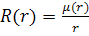
\includegraphics[width=67pt, height=27pt, keepaspectratio=true]{3-fig029.png}
{\large{}, получаем уравнение на }
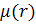
\includegraphics[width=27pt, height=19pt, keepaspectratio=true]{3-fig030.png}

\vspace{10pt}
%%\begin{figure}[htbp]
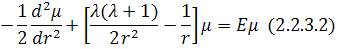
\includegraphics[width=254pt, height=37pt, keepaspectratio=true]{3-fig031.png}
%%\caption{This should be the caption for \texttt{3-fig031.png}.}
%%\end{figure}

\vspace{28pt}
{\large{}Уравнение имеет следующее решение}

\vspace{10pt}
%%\begin{figure}[htbp]
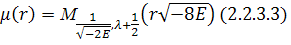
\includegraphics[width=218pt, height=34pt, keepaspectratio=true]{3-fig032.png}
%%\caption{This should be the caption for \texttt{3-fig032.png}.}
%%\end{figure}

\vspace{28pt}
{\large{}Энергия в этом выражении - величина, определяемая 
экспериментально.}

\vspace{10pt}
{\large{}Можно воспользоваться известной формулой 
}

\vspace{10pt}
%%\begin{figure}[htbp]
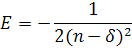
\includegraphics[width=99pt, height=37pt, keepaspectratio=true]{3-fig033.png}
%%\caption{This should be the caption for \texttt{3-fig033.png}.}
%%\end{figure}

\vspace{28pt}
{\large{}Тогда чтобы обеспечить сходимость }

\includegraphics[width=12pt, height=19pt, keepaspectratio=true]{3-fig034.png}
{\large{} - функции Уитеккера на бесконечности, 
}

\vspace{10pt}
%%\begin{figure}[htbp]
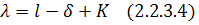
\includegraphics[width=149pt, height=19pt, keepaspectratio=true]{3-fig035.png}
%%\caption{This should be the caption for \texttt{3-fig035.png}.}
%%\end{figure}

\vspace{28pt}
%%\begin{figure}[htbp]

\includegraphics[width=11pt, height=19pt, keepaspectratio=true]{3-fig036.png}
%%\caption{This should be the caption for \texttt{3-fig036.png}.}
%%\end{figure}

 - 

\vspace{10pt}
{\large{}целое число}

\vspace{10pt}
{\large{}Обсудим более подробно проблему выбора 
K.}

\vspace{10pt}
{\large{}Т.к. при малых }{\large{}\textit{r}}{\large{} центростремительный 
член }
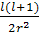
\includegraphics[width=29pt, height=27pt, keepaspectratio=true]{3-fig037.png}
{\large{} преобладает в }{\large{}\textit{V(r)}}{\large{}, Саймонс 
в оригинальной статье [10, стр. 646] предлагает 
определить }{\large{}\textit{K}}{\large{} таким образом, 
чтобы }
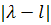
\includegraphics[width=38pt, height=19pt, keepaspectratio=true]{3-fig038.png}
{\large{} был минимальным.}

\vspace{10pt}
{\large{}Тогда }

\vspace{10pt}
%%\begin{figure}[htbp]
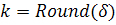
\includegraphics[width=87pt, height=19pt, keepaspectratio=true]{3-fig039.png}
%%\caption{This should be the caption for \texttt{3-fig039.png}.}
%%\end{figure}

\vspace{28pt}
%%\begin{figure}[htbp]
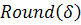
\includegraphics[width=61pt, height=19pt, keepaspectratio=true]{3-fig040.png}
%%\caption{This should be the caption for \texttt{3-fig040.png}.}
%%\end{figure}

 - 

\vspace{10pt}
{\large{}ближайшее к }

\includegraphics[width=8pt, height=19pt, keepaspectratio=true]{3-fig041.png}
{\large{} целое число.}

\vspace{10pt}
{\large{}В статье 1995 года [11, стр. 311] Мартин, довольно 
подробно обсуждая проблему выбора }

\includegraphics[width=8pt, height=19pt, keepaspectratio=true]{3-fig042.png}
{\large{}, указывает на то, что количество узлов 
радиальной функции равно }

\vspace{10pt}
%%\begin{figure}[htbp]
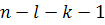
\includegraphics[width=79pt, height=19pt, keepaspectratio=true]{3-fig043.png}
%%\caption{This should be the caption for \texttt{3-fig043.png}.}
%%\end{figure}

\vspace{10pt}
{\large{}.}

\vspace{10pt}
{\large{}С математической точки зрения допустимы 
следующие значения }{\large{}\textit{k}}

\vspace{10pt}
%%\begin{figure}[htbp]
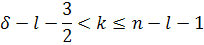
\includegraphics[width=153pt, height=34pt, keepaspectratio=true]{3-fig044.png}
%%\caption{This should be the caption for \texttt{3-fig044.png}.}
%%\end{figure}

\vspace{28pt}
{\large{}В качестве возможного выбора Мартин приводит 
}
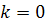
\includegraphics[width=34pt, height=19pt, keepaspectratio=true]{3-fig045.png}
{\large{}. В этом случае количество узлов в волновой 
функции такое же, как у соответствующей волновой 
функции атома водорода.}

\vspace{10pt}
{\large{}В собственной работе Мартин использует 
}
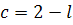
\includegraphics[width=55pt, height=19pt, keepaspectratio=true]{3-fig046.png}
{\large{} для }
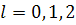
\includegraphics[width=57pt, height=19pt, keepaspectratio=true]{3-fig047.png}
{\large{}. В этом случае радиальная волновая функция 
при }
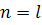
\includegraphics[width=32pt, height=19pt, keepaspectratio=true]{3-fig048.png}
{\large{} не имеет узлов.}

\vspace{10pt}
{\large{}В статье 2002 года [12, стр.75] Алчеев, также 
обсуждая проблему выбора k, использует для него 
следующее выражение.}

\vspace{10pt}
%%\begin{figure}[htbp]
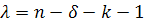
\includegraphics[width=108pt, height=19pt, keepaspectratio=true]{3-fig049.png}
%%\caption{This should be the caption for \texttt{3-fig049.png}.}
%%\end{figure}

\vspace{28pt}
{\large{}Алчеев определяет }

\includegraphics[width=8pt, height=19pt, keepaspectratio=true]{3-fig050.png}
{\large{} таким образом:}

\vspace{10pt}
%%\begin{figure}[htbp]
\includegraphics[width=136pt, height=19pt, keepaspectratio=true]{3-fig051.png}
%%\caption{This should be the caption for \texttt{3-fig051.png}.}
%%\end{figure}

\vspace{28pt}
%%\begin{figure}[htbp]
\includegraphics[width=17pt, height=19pt, keepaspectratio=true]{3-fig052.png}
%%\caption{This should be the caption for \texttt{3-fig052.png}.}
%%\end{figure}

 - 

\vspace{10pt}
{\large{}количество заполненных электронных оболочек.}

\vspace{10pt}
{\large{}Можно сделать вывод, что рассмотренные 
авторы определяют параметр k существенно по-разному, 
хотя результат расчета радиального матричного 
элемента может сильно зависеть от этого параметра.}

\newpage

\end{document}
